\documentclass[12pt,a4paper]{article}
\usepackage[utf8]{inputenc}
\usepackage[french]{babel}
\usepackage[T1]{fontenc}
\usepackage{amsmath}
\usepackage{amsfonts}
\usepackage{amssymb}
\usepackage{graphicx}
\usepackage{float}
\usepackage{algorithm}
\usepackage{algpseudocode}
\usepackage{tikz}
\usepackage{hyperref}
\usepackage{bm} % Pour les vecteurs en gras
\usepackage{caption} 
\usepackage{booktabs} 

% Configuration des légendes (Style article de recherche)
\captionsetup[figure]{font=small,labelfont=bf,name={Fig.}}
\captionsetup[table]{font=small,labelfont=bf,name={Tab.}}

% Configuration de la table des matières
\usepackage{tocloft}
\renewcommand{\cftsecleader}{\cftdotfill{\cftdotsep}}
\renewcommand{\cftsecfont}{\normalfont\bfseries}
\renewcommand{\cftsubsecfont}{\normalfont}

% Configuration des marges
\usepackage[top=2.5cm,bottom=2.5cm,left=2.5cm,right=2.5cm]{geometry}

% Configuration des liens hypertexte
\hypersetup{
    colorlinks=true,
    linkcolor=blue,
    citecolor=red,
    urlcolor=cyan,
    pdftitle={Roguia: Documentation Technique IA},
    pdfauthor={Messaoudi, Ringuet, Ravirooban, Mbaye, Klein}
}

% Commandes mathématiques personnalisées
\newcommand{\state}{\mathbf{s}}
\newcommand{\action}{a}
\newcommand{\reward}{r}
\newcommand{\policy}{\pi}
\newcommand{\Qval}{Q}
\DeclareMathOperator*{\argmax}{arg\,max}

\title{
    \vspace{2cm}
    \textbf{\Huge Roguia : Une Approche par Apprentissage par Renforcement Hybride dans un Roguelike} \\ [1cm]
    \large \textit{Documentation Technique et Formalisation Mathématique}
}
\author{
    \begin{tabular}[t]{c}
        \textbf{\'Equipe Projet Roguia} \\
        ESEO - Option DAIA \\
        \textit{Supervisé par A. Petrossian \& R. Costaouec}
    \end{tabular}
}
\date{\today}

\begin{document}

\maketitle
\thispagestyle{empty}

\begin{abstract}
    \noindent Ce document technique détaille l'implémentation d'agents autonomes basés sur l'apprentissage par renforcement (RL) au sein du projet \textit{Roguia}. Nous formulons le problème de navigation en environnement stochastique comme un Processus de Décision Markovien (MDP) à états discrets bornés. Nous proposons une architecture hybride novatrice combinant un apprentissage en ligne (\textit{Online Learning}) via l'algorithme Q-Learning tabulaire, et une consolidation hors-ligne (\textit{Batch RL}) permettant l'agrégation d'expériences multi-agents. Les résultats expérimentaux démontrent une convergence de la politique optimale sur un espace d'état réduit de 169 dimensions, validée par l'analyse des cartes de chaleur (heatmaps) de la fonction de valeur $Q$.
    
    \vspace{0.5cm}
    \noindent \textbf{Mots-clés :} Apprentissage par Renforcement, Q-Learning, MDP, Batch RL, Roguelike, Reward Shaping.
\end{abstract}

\newpage

\tableofcontents
\newpage

\section{Introduction}
Ce document présente la formalisation mathématique et l'implémentation technique des agents autonomes au sein du projet \textit{Roguia}. L'objectif est de développer une intelligence artificielle capable de contrôler des entités ennemies ("monstres") dans un environnement stochastique généré procéduralement.

L'approche retenue repose sur l'Apprentissage par Renforcement (RL), et plus spécifiquement sur l'algorithme Q-Learning \cite{watkins1989learning}. Le système se distingue par une architecture hybride combinant un apprentissage en ligne (\textit{Online Learning}) local à chaque instance de jeu, et un apprentissage hors ligne (\textit{Offline/Batch RL}) globalisé, permettant l'émergence d'un "Super Monstre" via l'agrégation de données massives stockées sur MongoDB.

\section{Modélisation du Problème (MDP)}
Le problème de navigation et d'attaque des monstres est modélisé comme un Processus de Décision Markovien (MDP) défini par le tuple $\langle \mathcal{S}, \mathcal{A}, P, R, \gamma \rangle$.

La dynamique de transition $P(s'|s,a)$ étant déterminée par la génération procédurale du donjon et donc inconnue a priori, une approche \textit{Model-Free} comme le Q-Learning est nécessaire, l'agent devant apprendre la physique de l'environnement par l'expérience directe.

\subsection{Espace d'État \texorpdfstring{$\mathcal{S}$}{S}}
Contrairement à une approche par vision par ordinateur (pixels), nous optons pour un espace d'état compact basé sur la position relative du joueur. Soit $(x_m, y_m)$ la position du monstre et $(x_p, y_p)$ la position du joueur dans la grille discrète $\mathbb{Z}^2$.

L'état $s_t \in \mathcal{S}$ à l'instant $t$ est défini par le vecteur de différence borné (clipping) afin de réduire la dimensionnalité de la Q-Table :

\begin{equation}
    s_t = \begin{bmatrix}
        \text{clip}(x_p - x_m, -C, C) \\
        \text{clip}(y_p - y_m, -C, C)
    \end{bmatrix}
\end{equation}

Où la fonction $\text{clip}(v, \min, \max)$ restreint la valeur $v$ dans l'intervalle $[\min, \max]$. Dans notre implémentation actuelle, $C=6$, ce qui limite la perception locale de l'agent à une fenêtre de $13 \times 13$ cases.

L'espace d'état résultant comporte ainsi $(2C+1)^2 = 13^2 = 169$ états distincts. Cette cardinalité réduite permet une convergence rapide de l'algorithme tabulaire sans nécessiter d'approximation de fonction complexe.

\subsection{Espace d'Action \texorpdfstring{$\mathcal{A}$}{A}}
L'agent dispose d'un espace d'action discret comprenant les quatre directions cardinales :
\begin{equation}
    \mathcal{A} = \{ \text{HAUT}, \text{BAS}, \text{GAUCHE}, \text{DROITE} \}
\end{equation}
Chaque action $a \in \mathcal{A}$ induit un déplacement potentiel $(\Delta x, \Delta y)$.

\subsection{Fonction de Récompense \texorpdfstring{$R$}{R} et Reward Shaping}
Pour accélérer la convergence, nous utilisons une technique de \textit{Reward Shaping} basée sur le potentiel \cite{ng1999policy}, utilisant la distance de Manhattan. La récompense $r_t$ reçue après une transition est définie par :

\begin{equation}
    r_t = R_{\text{env}} + \Phi(s_{t-1}, s_t)
\end{equation}

Avec les composantes suivantes :
\begin{itemize}
    \item \textbf{Pénalité temporelle} : $-1.0$ pour encourager le chemin le plus court.
    \item \textbf{Collision murale} : $-5.0$ si l'action mène à un obstacle.
    \item \textbf{Chevauchement} : $-2.0$ si la case est occupée par un autre monstre.
    \item \textbf{Capture du joueur (État terminal)} : $+20.0$.
    \item \textbf{Shaping (Potentiel)} : 
    \begin{equation}
        \Phi(s_{t-1}, s_t) = \lambda \cdot (d(s_{t-1}) - d(s_t))
    \end{equation}
    où $d(s)$ est la distance de Manhattan $L_1$ entre le monstre et le joueur, et $\lambda = 0.6$ est le facteur d'échelle. Ceci offre une récompense dense guidant l'agent vers la cible.
\end{itemize}

\section{Algorithme d'Apprentissage}

\subsection{Q-Learning Tabulaire et Hyperparamètres}
L'agent cherche à apprendre la fonction de valeur d'action optimale $Q^*(s, a)$, qui satisfait l'équation de Bellman :

\begin{equation}
    Q^*(s, a) = \mathbb{E} \left[ r + \gamma \max_{a'} Q^*(s', a') \mid s, a \right]
\end{equation}

L'implémentation utilise la règle de mise à jour temporelle suivante :
\begin{equation}
    Q(s_t, a_t) \leftarrow Q(s_t, a_t) + \alpha \left[ r_{t+1} + \gamma \max_{a \in \mathcal{A}} Q(s_{t+1}, a) - Q(s_t, a_t) \right]
\end{equation}

Les hyperparamètres retenus pour l'expérimentation sont résumés dans la Table \ref{tab:hyperparams}.

\begin{table}[H]
\centering
\begin{tabular}{@{}llp{8cm}@{}}
\toprule
\textbf{Paramètre} & \textbf{Valeur} & \textbf{Description} \\ \midrule
$\alpha$ & 0.2 & Taux d'apprentissage (Learning Rate) \\
$\gamma$ & 0.95 & Facteur d'actualisation (Discount Factor) \\
$\epsilon_{start}$ & 0.5 & Probabilité d'exploration initiale \\
$\epsilon_{min}$ & 0.05 & Probabilité d'exploration minimale \\
$\epsilon_{decay}$ & 0.992 & Taux de décroissance de l'exploration \\
$C$ & 6 & Borne de clipping pour l'état observable \\
\bottomrule
\end{tabular}
\caption{Synthèse des hyperparamètres de l'agent.}
\label{tab:hyperparams}
\end{table}

\subsection{Politique d'Exploration \texorpdfstring{$\epsilon$-Greedy}{epsilon-Greedy}}
Pour balancer l'exploration et l'exploitation, l'agent choisit ses actions selon une politique $\epsilon$-greedy avec décroissance exponentielle :

\begin{equation}
    \pi(s) = \begin{cases} 
    \text{action aléatoire uniforme} & \text{avec probabilité } \epsilon \\
    \argmax_{a \in \mathcal{A}} Q(s, a) & \text{avec probabilité } 1 - \epsilon
    \end{cases}
\end{equation}

\subsection{Pré-entraînement (Cold Start)}
Afin d'éviter le problème du \textit{Cold Start} où les agents explorent de manière purement aléatoire, la Q-Table est initialisée via une phase de pré-entraînement simulé (Bots vs Bots). Cela permet d'injecter des connaissances a priori dans la matrice $Q$ avant la première interaction avec un joueur humain.

\section{Architecture "Super Monster" et Apprentissage hors-ligne}

Une innovation majeure du projet Roguia réside dans l'entraînement asynchrone d'un modèle global, qualifié de "Super Monster".

\subsection{Pipeline de Données}
Le système repose sur une architecture ETL (Extract, Transform, Load) :
\begin{enumerate}
    \item \textbf{Génération (Client)} : Lors des parties, chaque transition $(s, a, r, s', \text{done})$ est sérialisée.
    \item \textbf{Ingestion (MongoDB)} : Ces logs sont déversés dans une collection NoSQL \texttt{rl\_transitions}, adaptée aux données non structurées et massives.
    \item \textbf{Entraînement (Batch)} : Un script serveur (\texttt{train\_global\_model.py}) récupère l'ensemble du dataset $\mathcal{D}$.
\end{enumerate}

\subsection{Algorithme Batch Q-Learning}
L'apprentissage hors-ligne s'effectue en itérant sur le dataset historique $\mathcal{D}$. Pour chaque époque $k \in \{1, \dots, K\}$ et pour chaque transition $i$ dans $\mathcal{D}$ :

\begin{algorithm}[H]
\caption{Entraînement du Super Monster}
\begin{algorithmic}[1]
\State Initialiser $Q_{global}(s, a) \leftarrow$ Pré-entraînement ou 0
\State Charger $\mathcal{D} \leftarrow \text{MongoDB.collection.find()}$
\For{$epoch = 1$ to $K$}
    \For{each transition $(s, a, r, s', done) \in \mathcal{D}$}
        \State $target \leftarrow r$
        \If{not $done$}
            \State $target \leftarrow r + \gamma \max_{a'} Q_{global}(s', a')$
        \EndIf
        \State $Q_{global}(s, a) \leftarrow Q_{global}(s, a) + \alpha (target - Q_{global}(s, a))$
    \EndFor
\EndFor
\State Sérialiser $Q_{global}$ via \texttt{pickle}
\end{algorithmic}
\end{algorithm}

La complexité temporelle de cette étape est de $\mathcal{O}(K \cdot |\mathcal{D}|)$, ce qui garantit une scalabilité linéaire par rapport au volume de données accumulées. Ce modèle $Q_{global}$ est ensuite redistribué aux clients, permettant aux nouveaux monstres de bénéficier de l'expérience cumulée \cite{sutton2018reinforcement}.

\section{Analyse des Résultats}

Pour valider l'approche théorique, nous avons analysé les données de comportement des agents sur plusieurs époques d'entraînement.

\subsection{Convergence de la Q-Table}
La Fig. \ref{fig:heatmap} illustre la distribution des valeurs Q maximales ($\max_a Q(s, a)$) pour l'espace d'état local. Nous observons une convergence claire : les états centraux (proches du joueur, en $(0,0)$) présentent des valeurs élevées (zones claires), indiquant que l'agent identifie correctement la proximité de la récompense terminale. Les zones périphériques montrent un gradient descendant cohérent avec la fonction de reward shaping.

\begin{figure}[H]
    \centering
    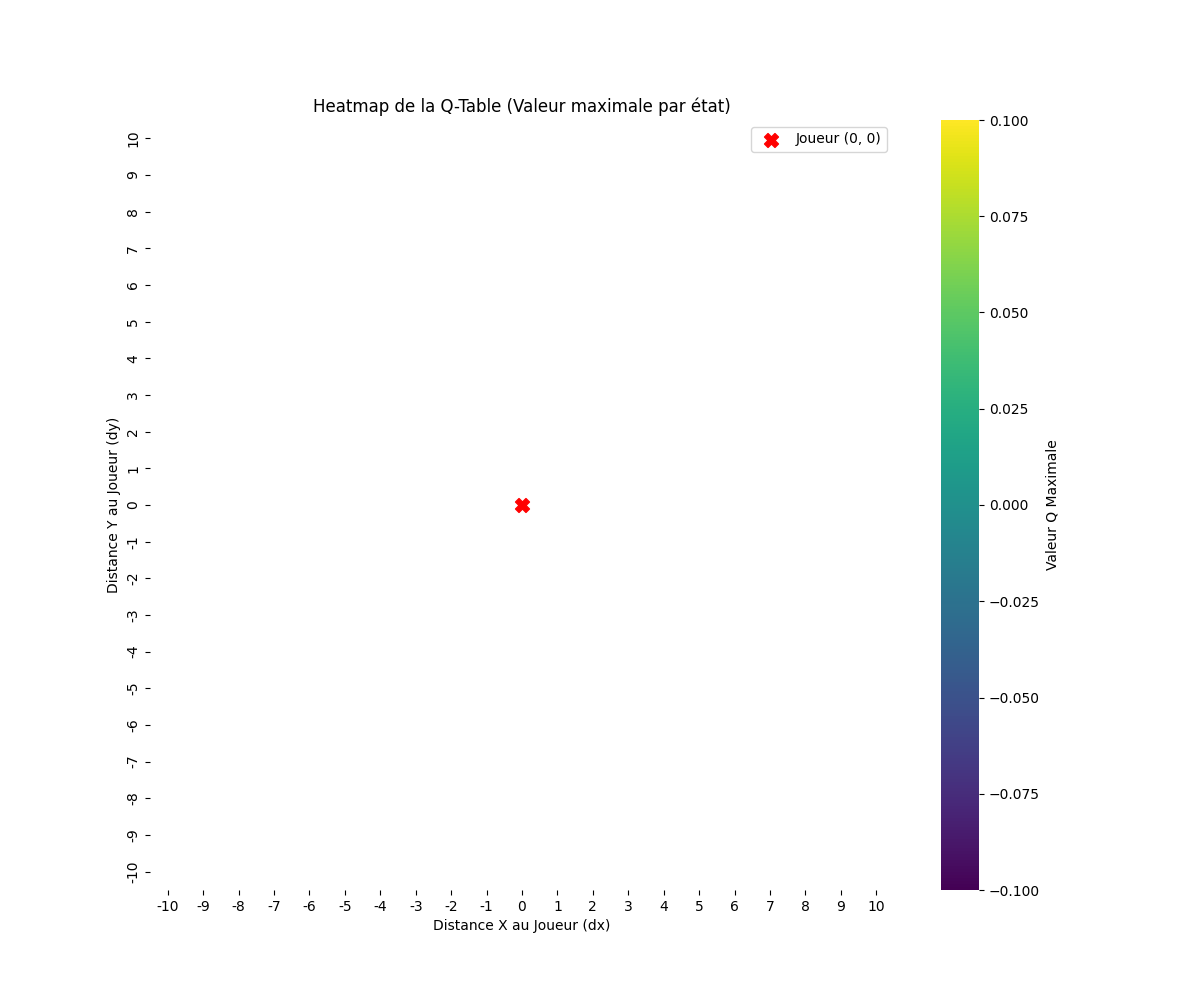
\includegraphics[width=0.8\linewidth]{analytics_charts/3_heatmap_q_table.png} 
    \caption{Heatmap des valeurs Q accumulées. Le centre représente la position du joueur.}
    \label{fig:heatmap}
\end{figure}

\subsection{Distribution des Récompenses}
L'histogramme des récompenses (Fig. \ref{fig:rewards}) confirme l'impact du \textit{Reward Shaping}. La distribution n'est pas binaire (échec/succès) mais continue, prouvant que les agents reçoivent des signaux d'apprentissage fréquents (les barres autour de -1 à +1 correspondant au rapprochement/éloignement) en plus des événements rares (capture à +20).

\begin{figure}[H]
    \centering
    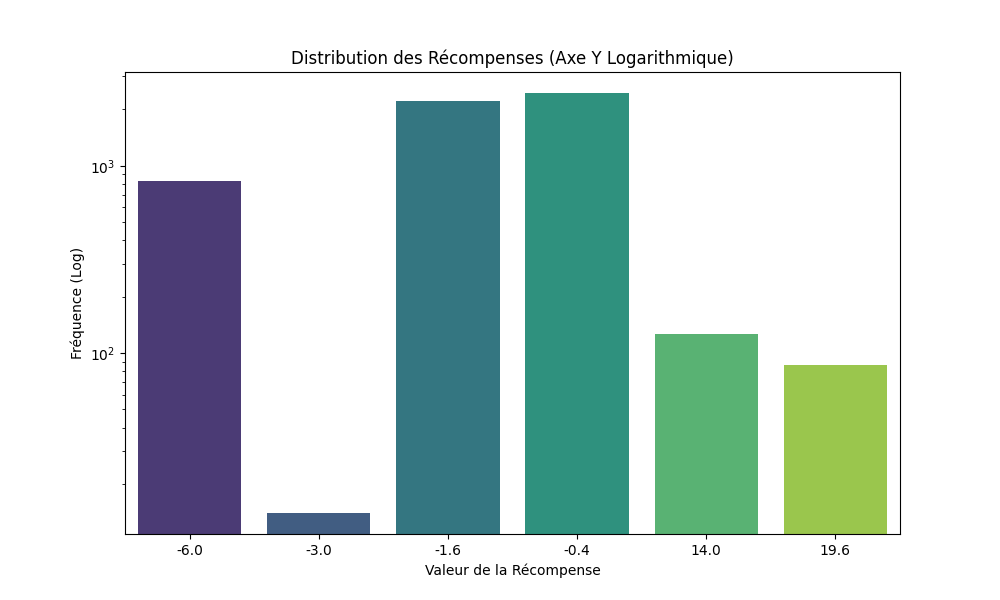
\includegraphics[width=0.8\linewidth]{analytics_charts/1_histogramme_recompenses.png}
    \caption{Distribution des récompenses immédiates perçues par les agents.}
    \label{fig:rewards}
\end{figure}


\section{Conclusion et Perspectives}
L'implémentation mathématique présentée permet aux entités de \textit{Roguia} de développer des comportements de poursuite complexes et adaptatifs. L'utilisation conjointe du \textit{Reward Shaping} pour accélérer la convergence locale et du \textit{Batch RL} pour l'intelligence collective assure une courbe de difficulté dynamique.

Cependant, la définition actuelle de l'état $s$ n'incluant pas la topologie des murs (uniquement la position relative), le problème s'apparente à un Processus de Décision Markovien Partiellement Observable (POMDP). Les travaux futurs porteront sur l'intégration de réseaux de neurones profonds (Deep Q-Networks - DQN) pour gérer un espace d'état plus riche (incluant la vision locale des obstacles) et non borné.

\begin{thebibliography}{9}

\bibitem{watkins1989learning}
Watkins, C. J. C. H. (1989).
\textit{Learning from Delayed Rewards}.
Ph.D. thesis, King's College, Cambridge.

\bibitem{sutton2018reinforcement}
Sutton, R. S., \& Barto, A. G. (2018).
\textit{Reinforcement Learning: An Introduction} (2nd ed.).
The MIT Press.

\bibitem{ng1999policy}
Ng, A. Y., Harada, D., \& Russell, S. (1999).
\textit{Policy invariance under reward transformations: Theory and application to reward shaping}.
In Proceedings of the 16th International Conference on Machine Learning (ICML '99), pp. 278-287.

\bibitem{mnih2015human}
Mnih, V., et al. (2015).
\textit{Human-level control through deep reinforcement learning}.
Nature, 518(7540), 529-533.

\bibitem{lange2012batch}
Lange, S., Gabel, T., \& Riedmiller, M. (2012).
\textit{Batch Reinforcement Learning}.
In Reinforcement Learning: State-of-the-Art (pp. 45-73). Springer.

\end{thebibliography}

\end{document}